\section{Processing Input}


\subsection{Lexical Analysis and Parsing}
nitially, input to PyPltRedex is read from the file and stored as a string. To apply reduction-relation, the string needs to be analyzed.

Lexical analysis breaks up the string into individual tokens and decides which kind of token it is. Most commonly tokens are described using regular expressions. 

Parsing takes individual lexemes and creates structured data out of them. In this case, it produces \texttt{Term} instances. 

The grammar can be seen in Figure \ref{tok-lex-grammar}.

\begin{figure}[h]
\begin{minted}[tabsize=2,obeytabs,escapeinside=::,mathescape=true,fontsize=\normalsize]{text}
term = term-sequence 
     | term-atom

term-sequence = lparen term* rparen

atom = (\#true|\#false|\#t|\#f)					  :$\langle boolean \rangle$:
	   | \"([^\"\\]|(\\[\s\S]))*\"				   :$\langle string  \rangle$:
	   | (\+|\-)?[0-9]*\.[0-9]+					    :$\langle float \rangle$:
	   | (\+|\-)?[0-9]+							        :$\langle integer \rangle$:
	   | ([^ \(\)\[\]\{\}\"\'`;\#\n])*
	     ([^ \(\)\[\]\{\}\"\'`;\#0123456789\n])+ 
	     ([^ \(\)\[\]\{\}\"\'`;\#\n])*       :$\langle identifier \rangle$:

lparen = [\[\{\(]             :$\langle opening \text{ } parentheses \rangle$:
rparen = [\]\}\)]             :$\langle closing \text{ } parentheses \rangle$:
\end{minted} 
\caption{Grammar for terms. All atoms match given regular expressions.}
\label{tok-lex-grammar}
\end{figure}

\subsection{Implementation}
Class diagram for both \texttt{Tokenizer} and \texttt{Parser} can be seen in Figure \ref{class-diagram-lexer-parser}.

\begin{figure}[h]
	\centering
	\makebox[\textwidth][c] { 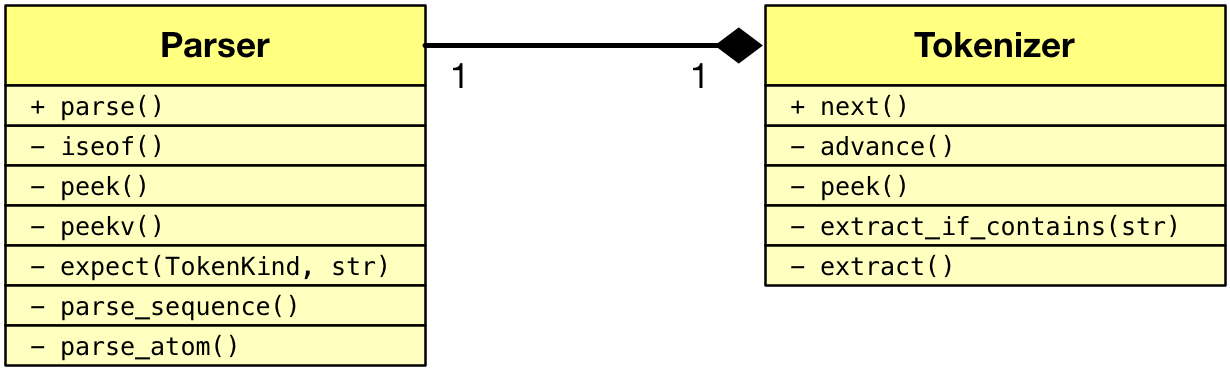
\includegraphics[scale=0.30]{class-diagram-lexer-parser.png} }
\caption{Class diagram for \texttt{Tokenizer} and \texttt{Parser}.}
\label{class-diagram-lexer-parser}
\end{figure}

The lexer implementation doesn't use regular expressions that were described above but implements their functionality using a manually implemented state machine. Functions that classify characters can be seen in Figure \ref{char-predicates}.

\begin{figure}[h]
\begin{minted}[tabsize=2,obeytabs,escapeinside=::,mathescape=true,fontsize=\normalsize]{python}
def is_whitespace(c):
    return c == ' ' or c == '\t' or c == '\n' or c == '\r'

def is_newline(c):
    return c == '\n'

def is_reserved(c): 
    return c in ['(', ')', '[', ']', '{', '}', '\"', '\'', '`', ';', '#', '|', '\\']

def is_digit(c):
    return c in ['0', '1', '2', '3', '4', '5', '6', '7', '8', '9']

def is_plusminus(c):
    return c in ['-', '+']

def is_delimeteter(c):
    return is_reserved(c) or c == '\0' or is_whitespace(c)

def is_leftparen(c):
	return c in ['(', '[', '{']

def is_rightparen(c):
	return c in [')', ']', '}']
\end{minted}
\caption{Predicates for character identification.}
\label{char-predicates}
\end{figure}


\begin{itemize}
\item
\texttt{string} is the string that requires lexical analysis.

\item
\texttt{start} and \texttt{end} are indices indicating an interval within the \texttt{string}. The substring that ends with index \texttt{start} has already been analyzed. A substring between \texttt{start} and \texttt{end} is a potential token. Any substring after \texttt{end} requires analysis.

\item
\texttt{advance()} method increments \texttt{end} by one.

\item
\texttt{peek()} returns a character at index \texttt{end} of the \texttt{string}.

\item
\texttt{extract\_if\_contains(substring)} extracts substring \texttt{s} beginning at \texttt{start} and ending at \texttt{start+len(substring)} and compares it against provided \texttt{substring}. If both strings are equal, \texttt{start} and \texttt{end} indices are set to \texttt{start+len(substring)} and True is returned. Otherwise, False is returned.

\item
\texttt{extract()} extracts the string between \texttt{start} and \texttt{end}, sets \texttt{start=end} and returns the extracted string.

\item
	\texttt{next()} returns the next token in the string. This method implements the tokenization logic. All regular expressions are implemented directly instead of using RPython's regular expression library (for reasons why see below). State machine representing this method can be seen in Figure \ref{lexical-analysis-tokenize}.

\begin{figure}[th!]
	\centering
	\makebox[\textwidth][c] { 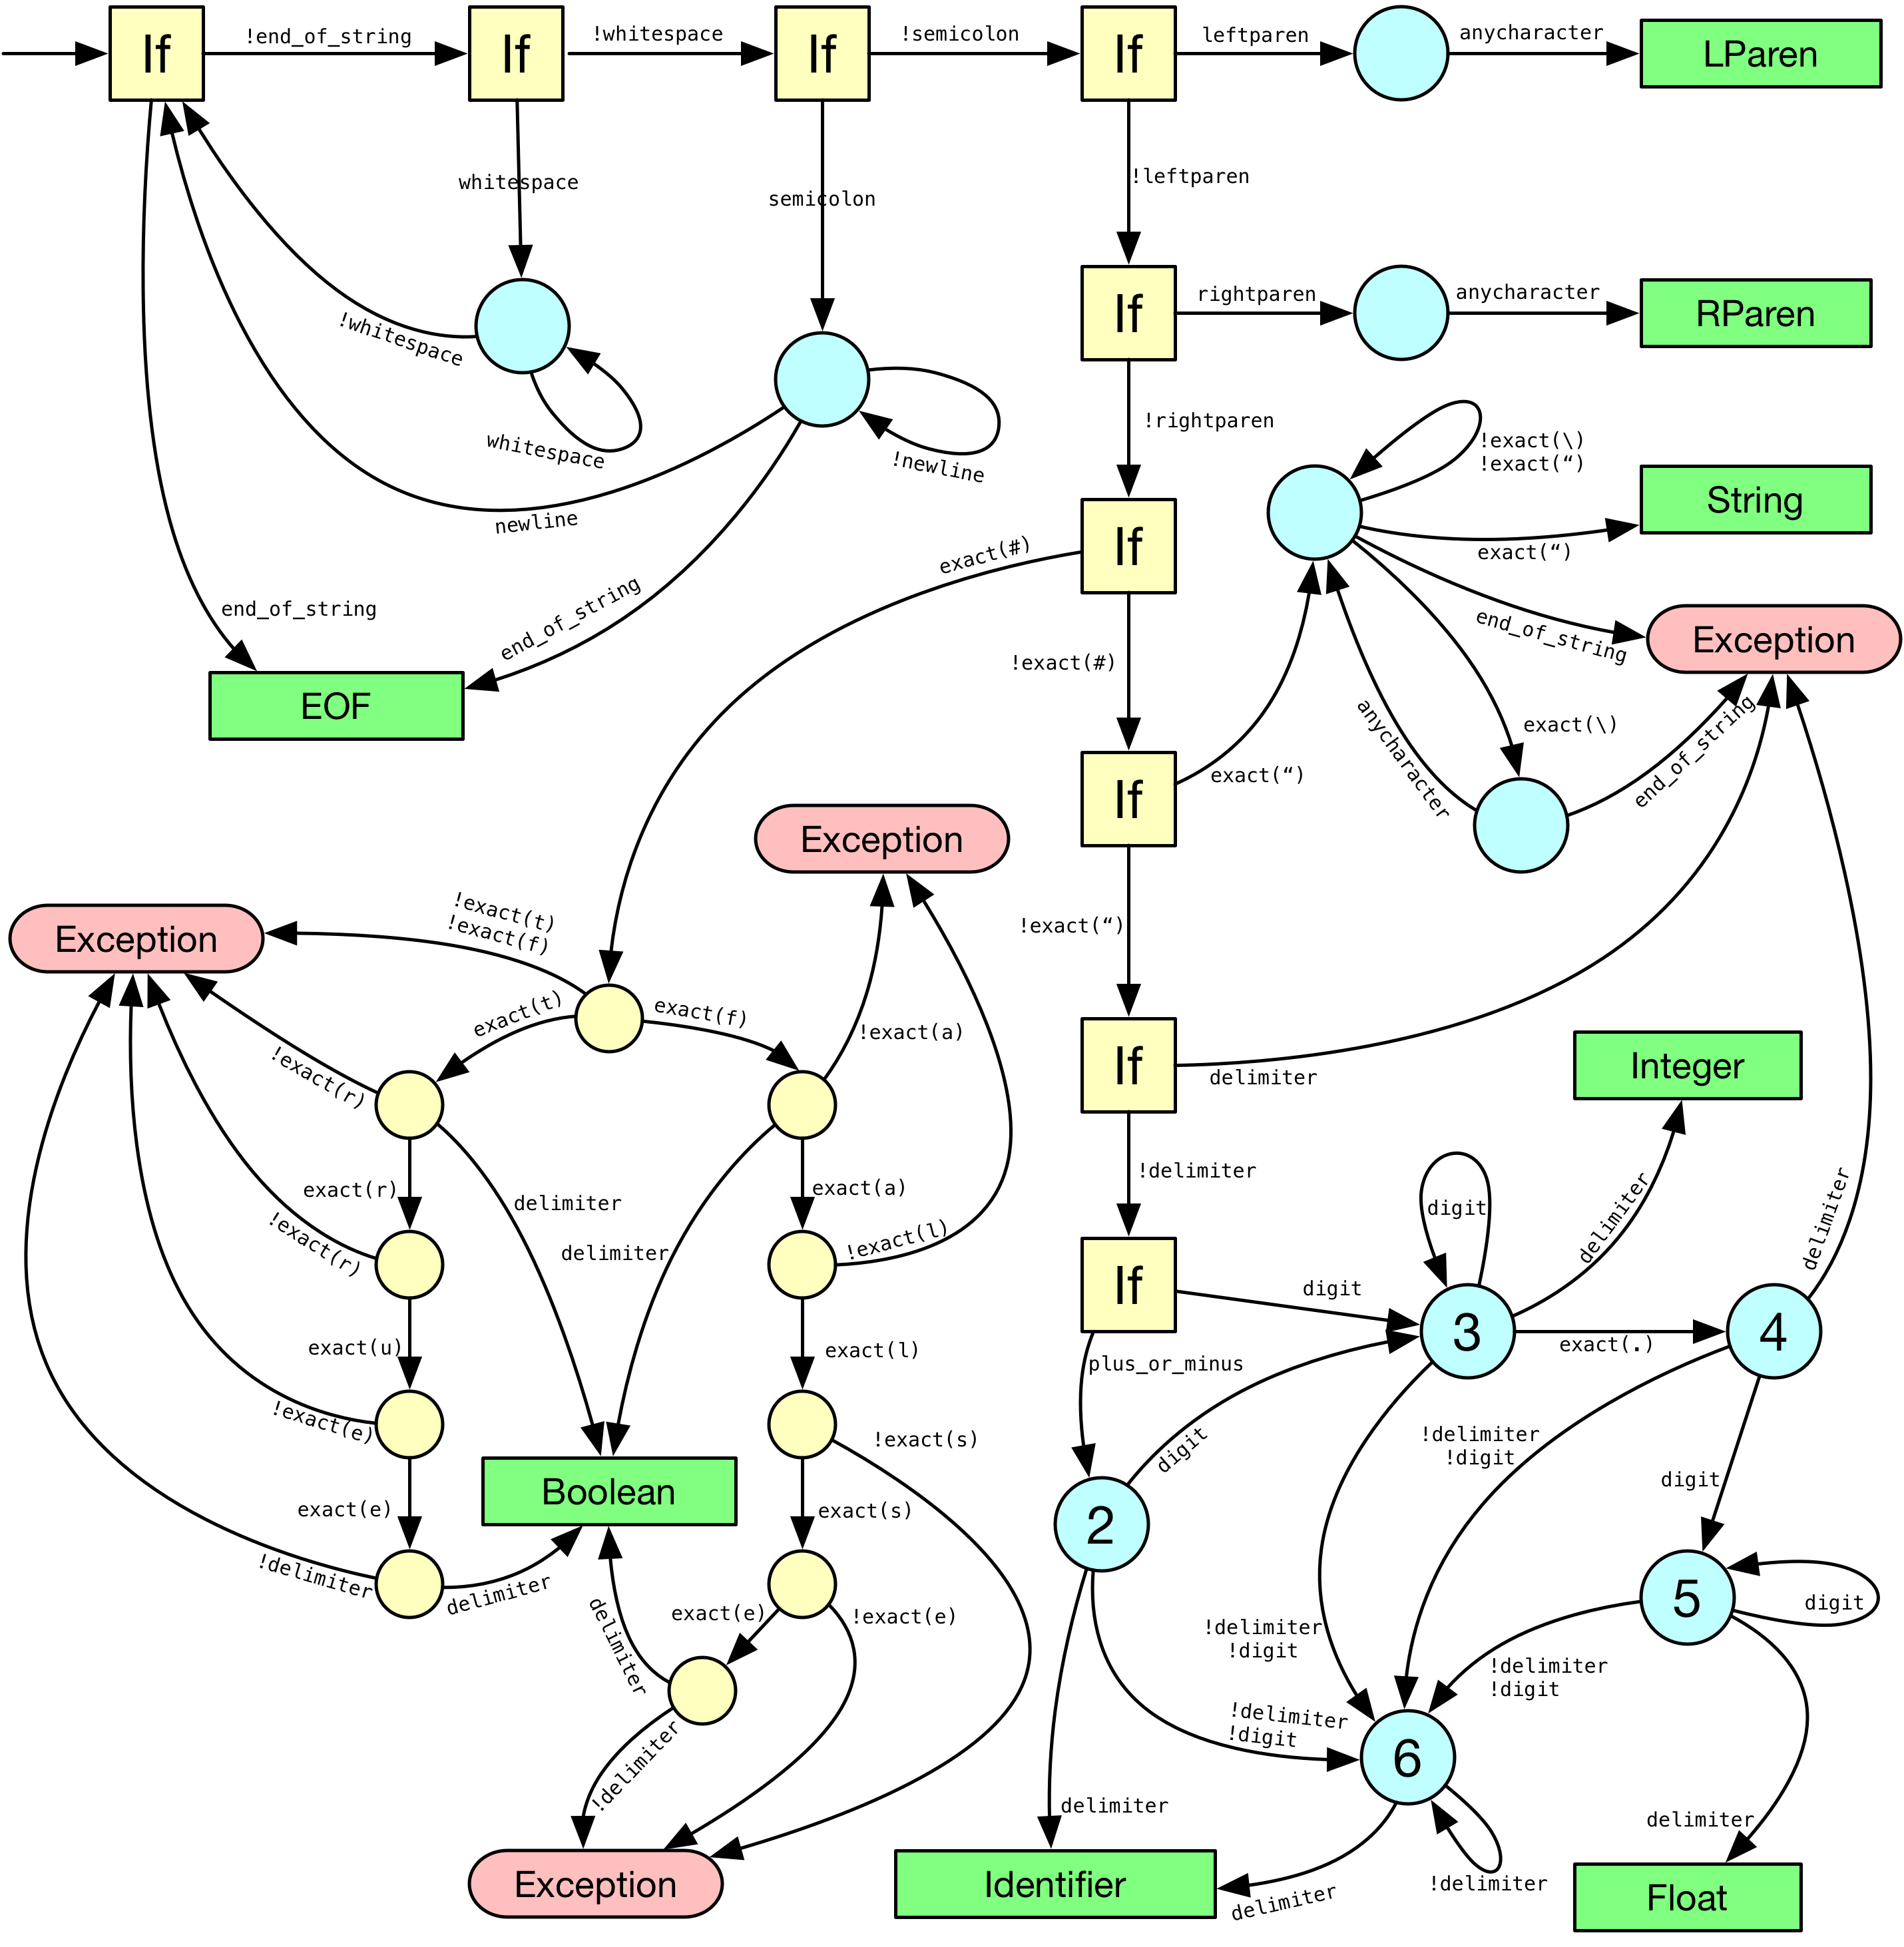
\includegraphics[scale=0.16]{lexical-analysis-tokenize.png} }
\caption{State machine for lexical analysis.}
\label{lexical-analysis-tokenize}
\end{figure}

Edges of the graph represent calls to \texttt{peek()} and ensure the character satisfies a predicate an edge is labeled with (see Figure \texttt{char-predicates}). Unlike more traditional state machines such as finite automatons in which moving from one state to another is associated with input consumption, the one above consumes input only after switching to some state. There are different state kinds which consume input in different ways.
\begin{itemize}
\item States that return tokens annotated with their types are highlighted in green. After moving to this state no input is consumed.
\item States that raise Exceptions are highlighted in red. After moving to this state no input is consumed.
\item \texttt{If} states correspond to \texttt{if} statements. They consume no characters.
\item Circled blue states actually consume characters that satisfy a predicate the incoming edge is labeled with. They can also have self-loops indicating consumption of one or more characters satisfying a given predicate.
\item Circled yellow states are conceptually identical to blue states but are handled differently as explained below.
\end{itemize}

The state machine proceeds in the following manner:

\begin{enumerate}
\item First it ensures the end of the string has not been reached, otherwise \texttt{EOF} token is returned. 
\item Then, if the current character is whitespace, greedily consume all whitespace characters and move to initial state.
\item If the current character is semicolon thus thus indicating the beginning of a comment, greedily consume all characters until newline or end of the string, thus returning \texttt{EOF} token. 
\item The next two If statements the detect opening and closing parantheses/braces/brackets and return \texttt{LParen} or \texttt{RParen} tokens accordingly.
\item If the current character starts with pound sign indicating a possible boolean, the transition to the yellow state would be taken. However, these yellow states do not consume input on character by character basis like blue states do but utilize \texttt{extract\_if\_contains} method to peek and consume multiple characters at once. This method is called in the following manner:
\begin{itemize}
\item
if \texttt{extract\_if\_contains("\#t")} return (Boolean "\#t)
\item
if \texttt{extract\_if\_contains("\#f")} return (Boolean "\#f)
\item
if \texttt{extract\_if\_contains("\#true")} return (Boolean "\#t)
\item
if \texttt{extract\_if\_contains("\#false")} return (Boolean "\#f)
\end{itemize}

\item If the current character is a double quote, consume any character until the closing double quote is found. Escape sequences are supported expecting a single character after a backward slash. If end-of-string is encountered prematurely, in Exception is raised. Otherwise, \texttt{String, self.extract()} token is returned.

\item Finally, the only token kinds remaining are \texttt{Integer}, \texttt{Float} and \texttt{Identifier}. First, need to ensure that the current character is not a special reserved one, raising an Exception. Otherwise, state machine moves to the last \texttt{If} statement. Explanation of state machine for these three token kinds would be too verbose to explain, but essentially it attempts to match an \texttt{Integer} or \texttt{Float} first but once a character that may not be in these two token kinds is seen, resulting token immediately becomes \texttt{Identifier}. All input from that point on is consumed greedly until some delimiter character.
\end{enumerate}

\end{itemize}

This completes the description of the tokenizer. The parser is implemented as a very simple recursive descent parser. Below follows the description of its methods and their functionalities.

\begin{itemize}
\item
\texttt{iseof()} returns true if the end of the string has been reached.

\item
\texttt{peek()} returns kind of the next token. 

\item
\texttt{peekv()} returns kind of the next token along with it's value.

\item 
\texttt{expect(expectedkind, tok=None)} throws Exception when \texttt{currenttoken} is not the one expected. In particular:
	\begin{itemize}
		\item
		If \texttt{expectedkind != nexttoken.kind}, raise an Exception.
		\item
		If \texttt{tok != None}, check if \texttt{tok=nexttoken.value} and raise an Exception if it is not.
		\item
		Otherwise, call \texttt{tokenizer.next()} and assign it to \texttt{nexttoken} and return the previous token. 
	\end{itemize}

\item 
	\texttt{parse\_sequence} implements parsing of \texttt{term-sequence} from the grammar above
	\begin{itemize}
		\item
		Let \texttt{seq} be an empty list.

		\item
		The first token is expected to be \texttt{LParen}.

		\item
		While \texttt{peek()} is not \texttt{RParen}, if \texttt{peek()} is \texttt{LParen}, call \texttt{term-sequence} and append its result to \texttt{seq}, otherwise call \texttt{parse\_atom} and append its result to \texttt{seq}.
	
		\item
		\texttt{expect(RParen)} and return \texttt{Sequence(seq)}
	\end{itemize}

\item
\texttt{parse\_atom} implements parsing of \texttt{atom} from grammar.
	\begin{itemize}
	\item
		If \texttt{peek()} is an \texttt{Integer} token, return \texttt{Integer(expect(Integer))}
	\item
		If \texttt{peek()} is a \texttt{Float} token, return \texttt{Float(expect(Decimal))}
	\item

		If \texttt{peek()} is a \texttt{String} token, return \texttt{String(expect(String))}
	\item
		If \texttt{peek()} is a \texttt{Boolean} token, return \texttt{Boolean(expect(Boolean))}
	\item

		If \texttt{peek()} is an \texttt{Ident} token, then call \texttt{peekv} to retrieve the \texttt{value} of the token. If \texttt{value} of token is \texttt{hole} return \texttt{Hole()}, otherwise \texttt{Variable(value)} is returned
	\end{itemize}
	

\end{itemize}

\subsection{Implementation: Difficulties}
The implementation of the initial lexical analysis relied on a regular expression library provided by RPython used to identify integers, floating point numbers and identifiers using regular expressions described in section TODO. While the library works fine while running the lexer using \texttt{python2.7}, attempting to compile the lexer code using \texttt{rpython} toolchain results in the following compilation error:

\begin{minted}[tabsize=2,obeytabs,fontsize=\normalsize]{python}
[translation:ERROR] AttributeError: 'FrozenDesc' object has no attribute 'pycall'
Processing block:
 block@1149[_choice5_0...] is a <class 'rpython.flowspace.flowcontext.SpamBlock'> 
 in (rpython.rlib.parsing.regexparse:1495)RegexParser._charclass 
 containing the following operations: 
       v1 = simple_call((type set), v0) 
       v2 = simple_call((builtin_function range), (97), (123)) 
       v3 = newlist() 
       v4 = iter(v2) 
       v5 = hint(v3, v2, ({'maxlength': True})) 
\end{minted}

There appears to be a bug within RPython's \texttt{RegexParser} functionality. After investigating the issue, it was decided to implement these regular expressions manually instead of relying on the library. This decision was also made because the construction of those regular expressions was rather slow.

\subsection{Future Improvements}

Since lexical analysis and parsing were implemented very early on, some of the regular expressions were hacked together to make everything work in short amount of time. In certain cases tokenization is not performed correctly with respect to Racket's tokenization logic. For example, Racket allows for specification of floating point numbers such as \texttt{.045} or \texttt{1.} (that is there must be either a digit before or after a decimal), which current implementation doesn't support (and are identified as Identifier instead). Scientific notation isn't supported, either.
